\documentclass[journal]{IEEEtran}
\usepackage{cite}
\usepackage{amsmath,amssymb,amsfonts}
\usepackage{algorithmic}
\usepackage{graphicx}
\usepackage{textcomp}
\usepackage{wrapfig}
\usepackage{caption}
\usepackage{subcaption}
\usepackage{enumitem}

\ifCLASSINFOpdf
\else
\fi

\hyphenation{op-tical net-works semi-conduc-tor}


\begin{document}
\title{IPA Project Report (Phase I) \\ Implementation of a 64-bit RISC-V CPU}


\author{
  \IEEEauthorblockN{Pavani Malchuru}
  \IEEEauthorblockA{(2024102043)} \\

  \IEEEauthorblockN{Nikhilesh Nallavelli} \\
  \IEEEauthorblockA{(2024102051)} \\

  \IEEEauthorblockN{Ritvik Avula} \\
  \IEEEauthorblockA{(2024112019)} \\
}

% The paper headers
\markboth{IPA Project Report}{RV64I CPU}

\maketitle

\begin{abstract}
  This report presents the design and implementation of a 64-bit RISC-V CPU
  using Verilog. We provide a comprehensive overview of the architecture used -
  from elaborating the design of each of the modules that constitute the CPU, to
  how the datapath was designed. For Phase 1, we implemented a CPU that
  processes instructions in a sequential order.
\end{abstract}


\section{Introduction and Background}

\IEEEPARstart{T}{he} RISC-V ISA is an open source instruction set architecture
that focuses on maintaining simple hardware and using basic instructions in
order to design and program more complicated entities. This simplicity makes
RISC-V an ideal choice for custom processor design. The instruction set is
modular, allowing implementations to support only the necessary base
instructions (RV64I) or extend with optional extensions for floating-point
operations, atomic instructions, and more. In this project, we focus on
implementing the RV64I base integer instruction set for 64-bit systems.

Of all the instructions in the base RV64I ISA, we've implemented the following
subset of instructions:

\begin{itemize}
  \item \textbf{R-type} (add, add/or/xor, sll/srl/sra)
  \item \textbf{I-type} (addi and etc..., ld, jalr)
  \item \textbf{S-type} (sd)
  \item \textbf{B-type} (beq)
  \item \textbf{J-type} (jal)
\end{itemize}

\section{Architecture and Design}

\begin{figure}[!ht]
  \centering
  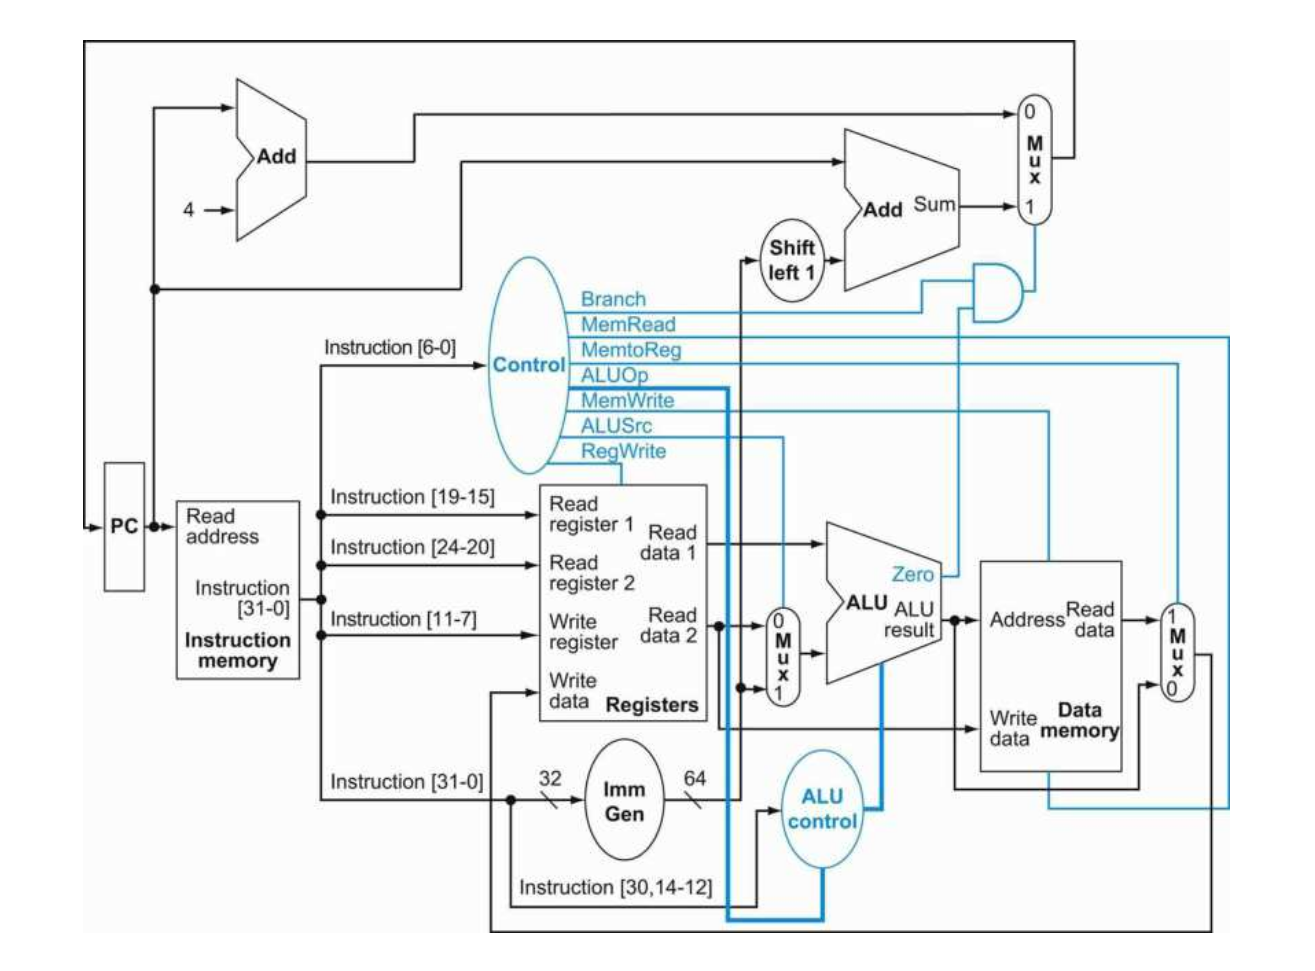
\includegraphics[width=0.45\textwidth]{figures/sequential_processor.png}
  \caption{High-level architecture of the RV64I sequential processor. Courtesy of \textit{Computer Organization and Design, Patterson and Hennessy}
    \cite{harris2021digital}}
  \label{fig:sequential_processor}
\end{figure}

The RV64I CPU consists of several key modules that work in conjunction to
execute instructions. Fig. \ref{fig:sequential_processor} illustrates the high-level
architecture of the processor.

The datapath consists of the following main components:

\begin{enumerate}
  \item \textbf{Program Counter (PC):} Stores the address of the current
        instruction and increments to fetch the next instruction
  \item \textbf{Instruction Memory:} Stores the program instructions
  \item \textbf{Register File:} Contains 32 general-purpose 64-bit registers
  \item \textbf{Arithmetic Logic Unit (ALU):} Performs computations - either
        arithmetic or to declare flags to be used in conditional operations
  \item \textbf{Control Unit:} Decodes and instruction and generates control
        signals that determine which modules should be active during the
        instruction cycle
  \item \textbf{Immediate Generator:} Extracts and extends immediate values from
        instructions
\end{enumerate}

The following subsections go into more detail about each of the modules.

\subsection{Program Counter (PC)}

\begin{description}[style=multiline, leftmargin=2cm, font=\bfseries]
  \item[Inputs:] \texttt{clk, reset, [63:0] pc\_in}
  \item[Outputs:] \texttt{[63:0] pc\_out}
\end{description}

The PC module manages instruction sequencing. It maintains the current program
counter value and implements control logic to either increment to the next
instruction or jump to a target address. The module is designed as a 64-bit
register with a synchronous update mechanism triggered by the clock.

\subsection{Instruction Memory}

\begin{description}[style=multiline, leftmargin=2cm, font=\bfseries]
  \item[Inputs:] \texttt{clk, reset, [63:0] pc\_curr}
  \item[Outputs:] \texttt{[31:0] inst}
\end{description}

The Instruction Memory module stores the program that we want to execute. These
instructions are 32 bits wide, and the current instruction is determined by the
value of the PC, which as discussed earlier, is 64 bits wide.

To function, the module first initializes its memory using instructions from the
file ```instructions.txt```, which has a byte of instruction per line - meaning
four lines in conjunction make up one specific instruction completely. The
module then reads instructions from instruction memory based on the current
PC value and outputs the fetched 32-bit instruction to the Control Block,
Register File, and the Immediate Generator.

\subsection{Register File}

\begin{description}[style=multiline, leftmargin=2cm, font=\bfseries]
  \item[Inputs:] \texttt{clk, reset, reg\_write\_en,} \\
        \texttt{[4:0] read\_reg1, read\_reg2, write\_reg,} \\
        \texttt{[63:0] write\_data}
  \item[Outputs:] \texttt{[63:0] read\_data1, read\_data2}
\end{description}

The register file contains 32 general-purpose 64-bit registers (x0 to x31),
where x0 is hardwired to zero. In general, the RISC-V registers are generally
assigned for the operations shown in Fig. \ref{fig:reg_file_convention}.

\begin{figure}[!ht]
  \centering
  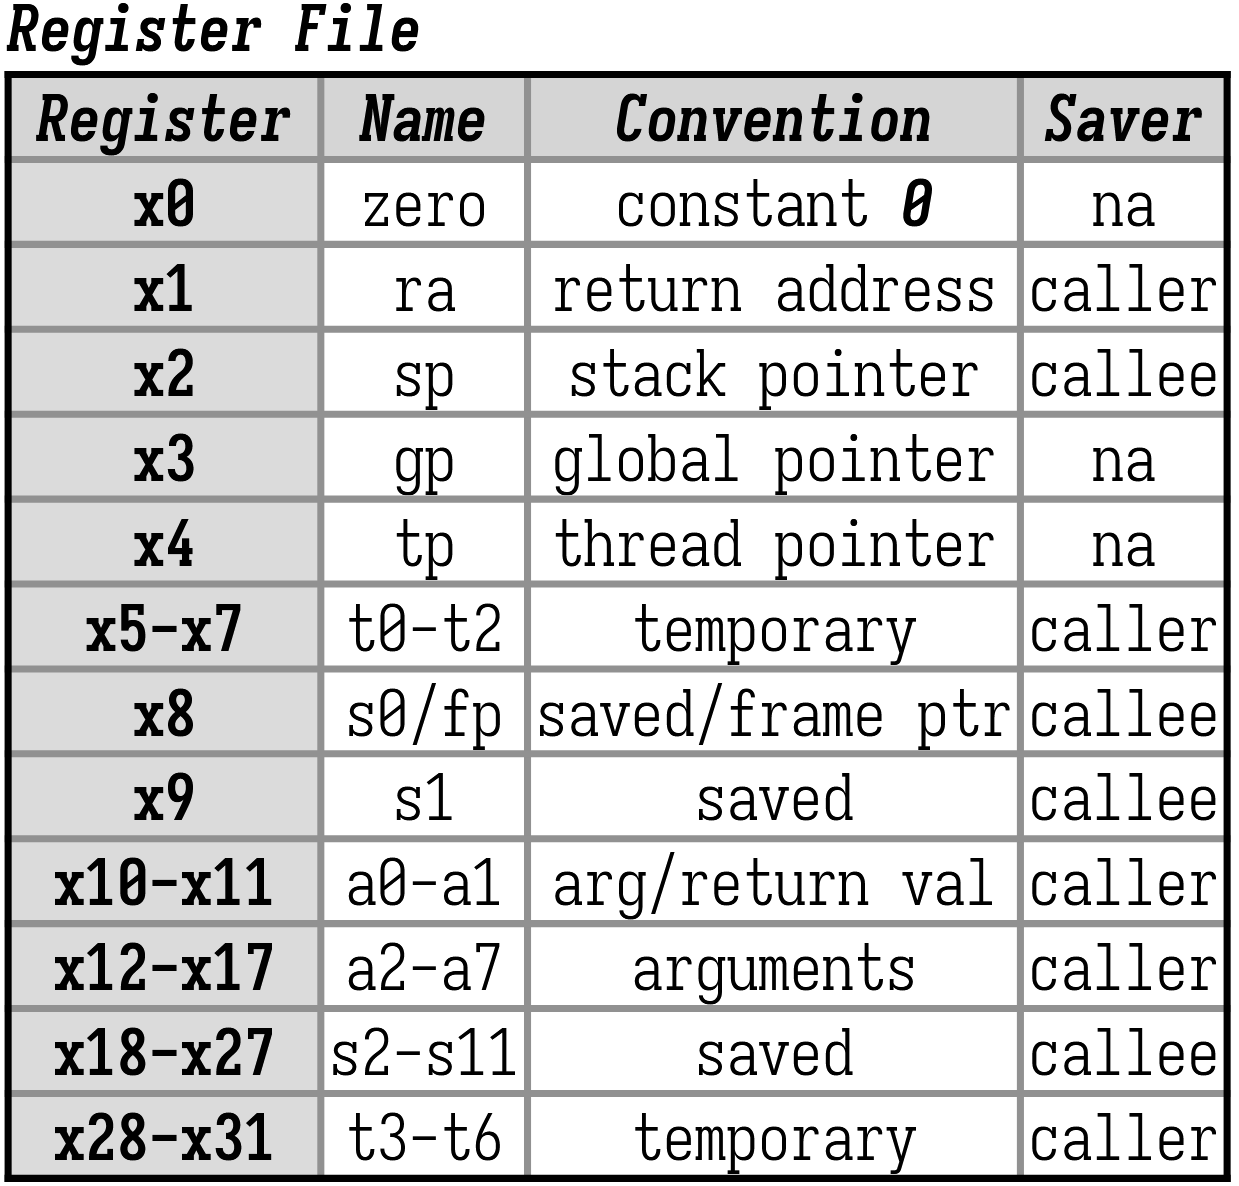
\includegraphics[width=0.45\textwidth]{figures/reg_file_convention.png}
  \caption{The RISC-V convention for how registers x0 to x31 are usually used.}
  \label{fig:reg_file_convention}
\end{figure}

The register file that we implemented has the following features.
\begin{itemize}
  \item Asynchronous dual-read ports for fetching operands
  \item One write port for storing results back in registers
  \item Control signals to enable/disable writing
\end{itemize}

To improve power efficiency, we implemented a 'lazy read' condition for x0 -
allowing writing to x0 but clearing it to 0 only when it's being read.

\subsection{Arithmetic Logic Unit (ALU)}

\begin{description}[style=multiline, leftmargin=2cm, font=\bfseries]
  \item[Inputs:] \texttt{[63:0] rs1, rs2} \\
        \texttt{[3:0] alu\_ctrl}
  \item[Outputs:] \texttt{[63:0] result,} \\
        \texttt{cout, carry\_flag, overflow\_flag, zero\_flag}
\end{description}

The ALU is a complex module responsible for executing arithmetic and logical
operations. The flags it generates are used for evaluating conditional
statements and determine validity of results. A brief description of the flags
is as follows:

\begin{itemize}
  \item \textbf{Carry flag:}  Indicates an unsigned overflow occurred during
        addition or subtraction. Set when the result exceeds the 64-bit range in
        unsigned arithmetic. Irrelevant for signed arithmetic.
  \item \textbf{Overflow flag:} Indicates a signed overflow occurred. Set when
        the result of a signed arithmetic operation exceeds the valid 64-bit
        signed range (-2\textsuperscript{63} to 2\textsuperscript{63}-1).
        Irrelevant for unsigned arithmetic.
  \item \textbf{Zero flag:} Set to 1 when the ALU result is zero. This is mainly
        used for conditional branch instructions (i.e, instructions like
        \texttt{beq}) to determine equality conditions.
\end{itemize}

An ALU is further constituted of a few major components of its own.

\subsubsection{64-bit Adder/Subtractor}
We used a ripple carry adder which can do both add and subtract operations. The
general structure is shown in Fig. \ref{fig:alu_adder}.

\begin{figure}[!ht]
  \centering
  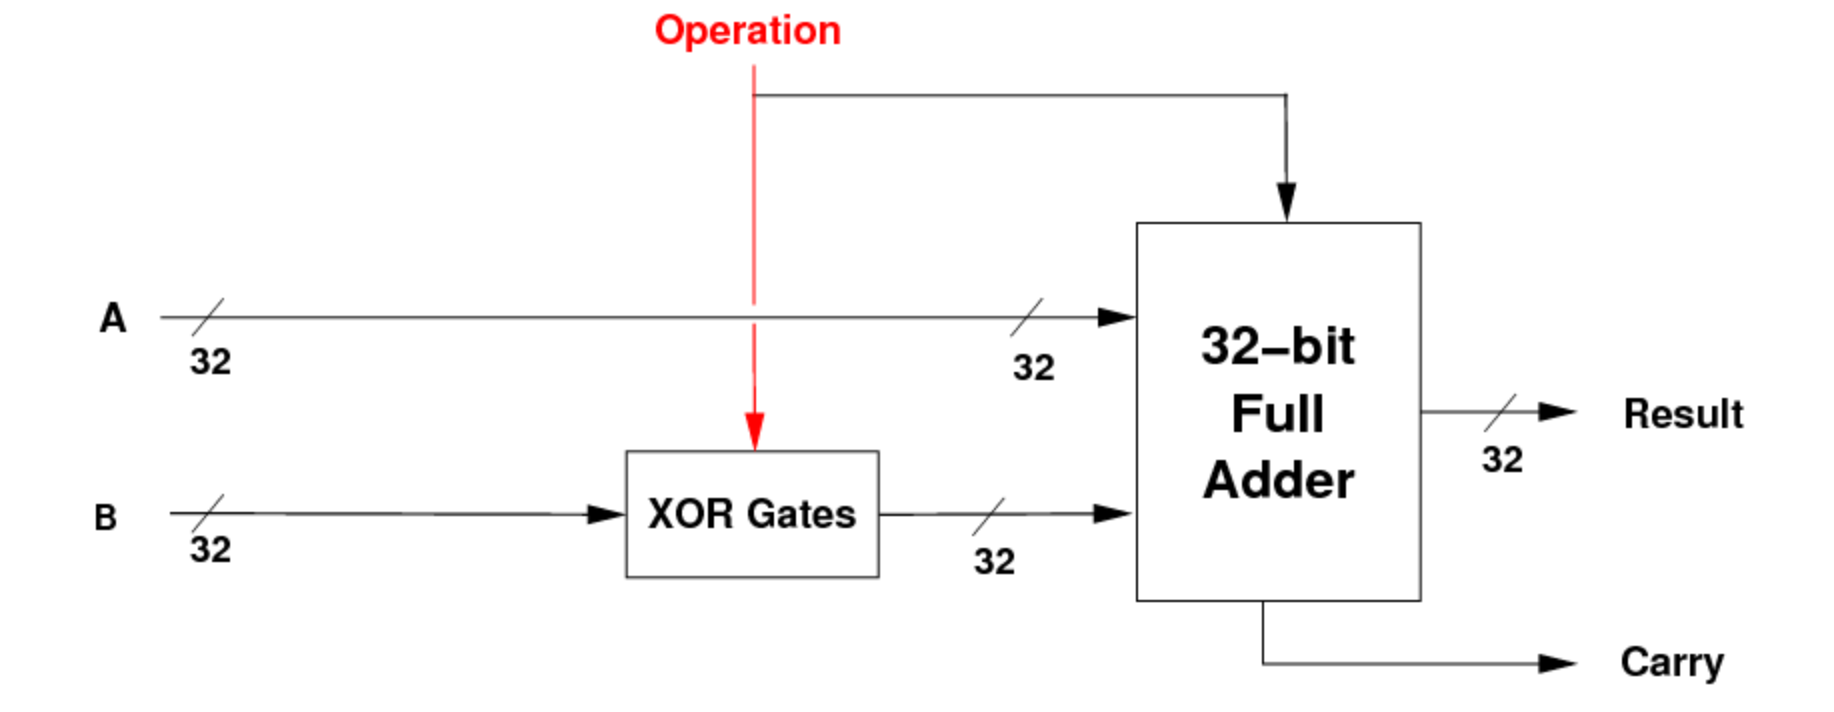
\includegraphics[width=0.45\textwidth]{figures/alu_adder.png}
  \caption{The adder block structure. The figure shows operation on 32-bit numbers, while we have extended it to 64 bits.}
  \label{fig:alu_adder}
\end{figure}

The cin input that is usually given to full adders is used here as an operation
selector; to replicate 2s complement subtraction, we do a + (!b) + 1.

\subsubsection{64-bit Logic Gates}
Implements bitwise logical operations like AND, OR, XOR, and NOR. Each operation is
performed bitwise across all 64 bits.

\subsubsection{64-bit Barrel Shifter}
Supports logical left shifts, logical right shifts, and arithmetic right shifts.
The shift amount is determined only by the least significant 6 bits of rs2
(allowing shifts up to 63 positions). Shifts above that are wrapped back - in
the sense that a bit shift of 64 bits would be the same as shifting by 1 bit.

Fig. \ref{fig:alu_adder} shows the general structure of a barrel shifter.

\begin{figure}[!ht]
  \centering
  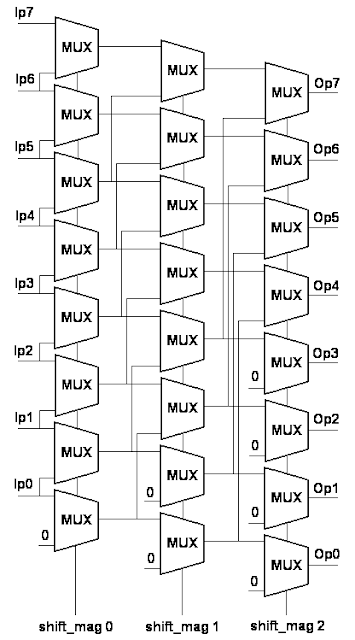
\includegraphics[width=0.45\textwidth]{figures/alu_barrel_shifter.png}
  \caption{A smaller 3x8 version of a barrel shifter. However, this does only left shifts.}
  \label{fig:alu_shifter}
\end{figure}

To generalize this for both right and left shifts, we implemented a row of muxes
before and after the circuit shown in Fig. \ref{fig:alu_shifter}. Based on the
opcode, the inputs would either be given in little endian or big endian format,
and collected at output likewise. This is because shifting right is technically
the same as shifting the bit-reversed input left.

Right shifts are also subdivided between logical and arithmetic shifts. To fix
this, instead of hardwiring the bottom muxes to zeros as shown in the figure, we
instead used the opcode to determine whether to give 0 (for logical shift)  or 1
(for arithmetic shift)

\subsection{Immediate Generator (Imm\_gen)}

This module extracts immediate values from the instruction and performs sign
extension to 64 bits. It handles multiple RISC-V instruction formats:
\begin{itemize}
  \item \textbf{I-type:} 12-bit signed immediates (instructions: ADDI, LW, etc.)
  \item \textbf{S-type:} 12-bit signed immediates (instructions: SW)
  \item \textbf{B-type:} 13-bit signed branch offsets (instructions: BEQ, BNE, etc.)
  \item \textbf{U-type:} 20-bit immediates shifted left by 12 bits (instructions: LUI)
  \item \textbf{J-type:} 21-bit signed jump offsets (instruction: JAL)
\end{itemize}

\subsection{Control Units}

Two control modules coordinate instruction execution:

\subsubsection{Main Control Unit (MCU)}
Decodes the 7-bit opcode field of the instruction and generates high-level
control signals such as:
\begin{itemize}
  \item ALU operation selection
  \item Register file write enable
  \item Data path multiplexing controls
  \item Memory access controls (for future phases)
\end{itemize}

\subsubsection{ALU Control Unit}
Takes the 3-bit funct3 field and 7-bit funct7 field from the instruction and
generates 4-bit ALU function codes. This implements the secondary decoding layer
required for instructions with multiple variants.

\section{Implementation Details}

\subsection{Module Interfaces}

All modules are designed with clear input/output interfaces to enable modular
testing and integration:

\begin{itemize}
  \item Modules use consistent 64-bit data widths for operands and results
  \item Control signals are clearly named to indicate their function
  \item Clock and reset signals are provided to all sequential components
  \item Each module can be independently tested with dedicated testbenches
\end{itemize}

\subsection{Instruction Set Support}

The Phase 1 implementation supports a subset of RV64I base instructions,
including:
\begin{itemize}
  \item \textbf{Arithmetic:} ADD, ADDI, SUB, SUBI
  \item \textbf{Logic:} AND, ANDI, OR, ORI, XOR, XORI
  \item \textbf{Shift:} SLL, SLLI, SRL, SRLI, SRA, SRAI
  \item \textbf{Load/Store:} LW, SW (basic support)
\end{itemize}

\section{Testing and Verification}

Each module includes comprehensive testbenches written in Verilog to verify
correct operation:

\subsection{Individual Module Testing}

Testbenches have been developed for each functional module:
\begin{itemize}
  \item \textbf{ALU Testbench:} Verifies all arithmetic operations, logic operations, and shift operations with various input patterns
  \item \textbf{Adder64 Testbench:} Tests 64-bit addition and subtraction with edge cases including overflow scenarios
  \item \textbf{Gate64 Testbench:} Validates bitwise logic operations
  \item \textbf{Shift64 Testbench:} Confirms correct shifting behavior for all shift types
  \item \textbf{Register File Testbench:} Tests read and write operations across all registers
  \item \textbf{Immediate Generator Testbench:} Validates immediate extraction and sign extension for all instruction formats
  \item \textbf{Control Unit Testbench:} Verifies opcode decoding and control signal generation
  \item \textbf{PC Testbench:} Tests program counter increment and branch handling
\end{itemize}

\subsection{Test Coverage}

The testbenches include:
\begin{itemize}
  \item Normal operation cases with representative inputs
  \item Edge cases such as zero operands, maximum values, and boundary conditions
  \item Negative operands to verify sign handling
  \item Cross-module integration tests to ensure correct communication
\end{itemize}

\subsection{Simulation and Results}

Simulations are performed using Icarus Verilog, with waveform outputs captured
in .vcd format for detailed analysis of signal behavior. The
simulation results confirm correct operation of all modules within their
specified functional requirements.

\section{Challenges and Solutions}

\subsection{64-bit Arithmetic}
Implementing correct carry propagation in the 64-bit adder required careful
attention to the ripple-carry logic to ensure timing closure.

\subsection{Instruction Format Decoding}
The varying formats of RISC-V instructions necessitated a flexible immediate
generator that correctly extracts and sign-extends immediates based on
instruction type.

\subsection{Control Signal Coordination}
Synchronizing control signals across multiple modules required careful design of
the control unit hierarchy to avoid hazards.

\section{Future Work (Phase 2)}

While Phase 1 establishes the foundational architecture, Phase 2 will extend the
design with:
\begin{itemize}
  \item Data memory module for load/store operations
  \item Pipeline stages (fetch, decode, execute, memory, writeback)
  \item Hazard detection and forwarding logic
  \item Branch prediction mechanisms
  \item Additional instruction set extensions (multiply, divide, etc.)
\end{itemize}

\section{Conclusion}

This project successfully demonstrates the design and implementation of a 64-bit
RISC-V processor core. The modular architecture allows for clear separation of
concerns and facilitates future extensions. All modules have been thoroughly
tested and verified to operate correctly. The Phase 1 design provides a solid
foundation for implementing a pipelined processor in subsequent phases.

\ifCLASSOPTIONcaptionsoff
  \newpage
\fi

\bibliographystyle{IEEEtran}
\nocite{*}
\bibliography{references.bib}

\end{document}


